\onecolumn
\chapter{Auswertung}
\label{ch:auswertung}

\section*{Fehlerrechnung}
Für die statistische Auswertung von $n$ Messwerten $x_i$ werden folgende Größen definiert \cite{errorSkript25}:
\begin{align}
    \bar{x} &= \frac{1}{n} \sum_{i=1}^{n} x_i \vphantom{\sqrt{\sum_i^n}^2} && \text{\textcolor{gray}{Arithmetisches Mittel}} \label{eq:arithmetisches_mittel} \\
    \sigma^2 &= \frac{1}{n-1} \sum_{i=1}^{n} (x_i - \bar{x})^2 \vphantom{\sqrt{\sum_i^n}^2} && \text{\textcolor{gray}{Variation}} \label{eq:variation} \\
    \sigma &= \sqrt{\frac{1}{n-1} \sum_{i=1}^{n} (x_i - \bar{x})^2} \vphantom{\sqrt{\sum_i^n}^2} && \text{\textcolor{gray}{Standardabweichung}} \label{eq:standardabweichung} \\
    \Delta \bar{x} &= \frac{\sigma}{\sqrt{n}} = \sqrt{\frac{1}{n(n-1)} \sum_{i=1}^n(\bar x - x_i)^2} \vphantom{\sqrt{\sum_i^n}^2} && \text{\textcolor{gray}{Fehler des Mittelwerts}} \label{eq:fehler_mittelwert} \\
    \Delta f &= \sqrt{\left(\frac{\partial f}{\partial x} \Delta x\right)^2 + \left(\frac{\partial f}{\partial y} \Delta y\right)^2} \vphantom{\sqrt{\sum_i^n}^2} && \text{\textcolor{gray}{Gauß’sches Fehlerfortpflanzungsgesetz für $f(x,y)$}} \label{eq:gauss_fehlfortpflanzung} \\
    \Delta f &= \sqrt{(\Delta x)^2 + (\Delta y)^2} \vphantom{\sqrt{\sum_i^n}^2} && \text{\textcolor{gray}{Fehler für $f = x + y$}} \label{eq:fehler_summe} \\
    \Delta f &= |a| \Delta x \vphantom{\sqrt{\sum_i^n}^2} && \text{\textcolor{gray}{Fehler für $f = ax$}} \label{eq:fehler_proportional} \\
    \frac{\Delta f}{|f|} &= \sqrt{\left(\frac{\Delta x}{x}\right)^2 + \left(\frac{\Delta y}{y}\right)^2} \vphantom{\sqrt{\sum_i^n}^2} && \text{\textcolor{gray}{relativer Fehler für $f = xy$ oder $f = x/y$}} \label{eq:relativer_fehler} \\
    \sigma &= \frac{|a_{lit} - a_{gem}|}{\sqrt{\Delta a_{lit}^2 + \Delta a_{gem}^2}} \vphantom{\sqrt{\sum_i^n}^2} && \text{\textcolor{gray}{Berechnung der signifikanten Abweichung}} \label{eq:signifikante_abweichung}
\end{align}

\twocolumn


% //////////////// Aufgabe 1 ////////////////
\section{Aufgabe 1: Spannungsmessung mit verschiedenen Messgeräten}
In dieser Aufgabe soll die Spannung der Batterie sowie die Spannungen an den beiden Widerständen des Spannungsteilers gemessen werden. Dabei werden die Messungen sowohl mit dem als Voltmeter betriebenen Drehspulinstrument als auch mit dem Kompensator durchgeführt. Ziel ist es, den Einfluss des Innenwiderstands des Drehspulinstruments auf die Messergebnisse zu untersuchen. 
Die Werte sind dem \hyperref[Protokoll]{Protokoll} zu entnehmen. Dabei ist Tabelle 1 für die Messwerte des Drehspulinstruments und Tabelle 2 für die Messwerte des Kompensators zu beachten.

% ------ Drehspulinstument ------
\subsection*{Drehspulinstrument}
Der Innenwiderstand des Messgerätes wird über die Summe der Widerstände des Dekadenwiderstands $R_s$ und des Widerstands des Drehspulinstruments $R_V$ bestimmt:
\begin{equation}   
    R_{sV} = R_s + R_V
    \label{eq:innenwiderstand_voltmeter}
\end{equation}
Der Rechnug des Protokolles sind die Widerstandswerte zu entnehmen. Aus diesen bestimmt sich der Innenwiderstand des als Voltmeter betriebenen Drehspulinstruments zu:
\begin{equation}
    R_{sV} = 442\Omega + 58\Omega = 500\Omega.
\end{equation}

Aus der \hyperref[eq:ohm]{Gleichung \ref*{eq:ohm}} folgt für die Spannung am Voltmeter:
\begin{equation}
    U_V = R_{sV} \cdot I.
    \label{eq:spannung_voltmeter}
\end{equation}

Der Fehler des Innenwiderstands wird über die \hyperref[eq:fehler_summe]{Gleichung \ref*{eq:fehler_summe}} bestimmt:
\begin{equation}
    \Delta R_{sV} = \sqrt{( \Delta R_s )^2 + ( \Delta R_V )^2}
\end{equation}
mit $\Delta R_s = 0,2\% \cdot R_s$ und $\Delta R_{V} = 1\% \cdot R_V$. Damit ergibt sich:
\begin{equation}
    \Delta R_{sV} = 4,42\Omega.
\end{equation}

Der Fehler der Stromstärke setzt sich aus dem Ablesefehler des Drehspulinstruments von $\Delta I = 0,5 \cdot 0,2mA$ und und dem Fehler des MEssgreätes selbst $R_V = 0,25mA$ zusammen. Über die \hyperref[eq:fehler_summe]{Gleichung \ref*{eq:fehler_summe}} ergibt sich damit:
\begin{equation}
    \Delta I = 0,3mA.
    \label{eq:fehler_strom}
\end{equation}

Die Spannung am Voltmeter wird über die \hyperref[eq:spannung_voltmeter]{Gleichung \ref*{eq:spannung_voltmeter}} berechnet. Der Fehler der Spannung wird über die \hyperref[eq:gauss_fehlfortpflanzung]{Gleichung \ref*{eq:gauss_fehlfortpflanzung}} bestimmt:
\begin{equation}
    \Delta U_V = \sqrt{(I \cdot \Delta R_{sV})^2 + (R_{sV} \cdot \Delta I)^2}.
\end{equation}

Folglich ergeben sich die Spannungen und deren Fehler der Batteriespannung $U_0$ zu:
\begin{equation}
    \boxed{
        U_0 = (4,85 \pm 0,16) \, V
    }
\end{equation}

Für die Spannung über den Widerstand $R_1$ ergibt sich:
\begin{equation}
    \boxed{
        U_{R} = (1,20 \pm 0,13) \, V
    }
\end{equation}

Für die Spannung über den Widerstand $R_2$ ergibt sich dieselbe Spannung. Es ist zu beachten, dass die Summe der Spannungen über den Widerständen nicht exakt der Batteriespannung entspricht. Dies ist auf den Einfluss des Innenwiderstands des Messgerätes zurückzuführen. Nach \hyperref[eq:spannunglast]{Gleichung \ref*{eq:spannunglast}} gilt für die Batteriespannung:
\begin{equation}
    U_0 = \frac{U_q \cdot 2R}{R_s + 2R +\frac{R_1 \cdot R}{R_{sV}}}
\end{equation}

und für die Spannung über die Widerstände $R_1$ und $R_2$:
\begin{equation}
    U_{R} = \frac{U_q \cdot R}{R_s + 2R +\frac{R_1 \cdot R}{R_{sV}} +\frac{R^2}{R_{sV}}}.
\end{equation}

Dies ist die Spannung pro Widerstand, da beide Widerstände gleich groß sind. Die Gesamtspannugn ist somit $2U_R$. Dies zeigt, dass die Summe der Spannungen über den Widerständen kleiner als die Batteriespannung ist, was den Messergebnissen entspricht. Um genau zu sein, unterscheiden sich die Spannungen um den Therm im Nenner von $\frac{R^2}{R_{sV}}$. Dieser Therm verschwindet für einen im wesentlichen größe Innenwiderstand des Messgerätes, als Lastwiderstände ($R_{sV} \gg R_V$).
Weitergehend soll die Stromstärke $I_0$ über die Krischhoff'sche Knotenregel (\hyperref[eq:knoten]{Gleichung \ref*{eq:knoten}}) bestimmt werden. Dabei gilt:
\begin{equation}
    I_0 = I_V + I_{R1} + I_{R2}
\end{equation}
wobei $I_V$ die Stromstärke durch das Voltmeter und $I_{R1}$ und $I_{R2}$ die Stromstärken durch die Widerstände $R_1$ und $R_2$ sind. Diese werden über die \hyperref[eq:ohm]{Gleichung \ref*{eq:ohm}} bestimmt. Da $R_1 = R_2$ gilt, wird die Summe asl $R$ geschrieben. Damit folgt:
\begin{equation}
    I_0 = \frac{U_V}{R_{sV}} + 2 \cdot \frac{U_R}{R}.
\end{equation}

Wobei gilt:
\begin{equation}
    I_0 = \frac{U_0}{R_{ges}}
\end{equation}
mit dem Gesamtwiderstand
\begin{equation}
    R_{ges} = \frac{R_{sV} \cdot R}{R_{sV} + R} + R.
\end{equation}

Alles zusammengefasst und nach $R$ umgestellt ergibt:
\begin{equation}
    R = \left( \frac{U_0}{U_R} - 2 \right) \cdot R_{sV} = 1020,84\Omega.
\end{equation}

Nach \hyperref[eq:gauss_fehlfortpflanzung]{Gauß'scher Fehlerfortpflanzung (\ref*{eq:gauss_fehlfortpflanzung})} ergibt sich der Fehler zu:
\begin{align}
    \Delta R = \sqrt{
        \begin{aligned}
            &\left(\frac{R_{sV}}{U_R} \Delta U_0 \right)^2 
            + \left( \frac{U_0 \cdot R_{sV}}{U_R^2} \Delta U_R \right)^2 \\
            &+ \left( \left( \frac{U_0}{U_R} - 2 \right) \Delta R_{sV} \right)^2
        \end{aligned}
    }
\end{align}


Folglich ergibt sich für den Widerstand:
\begin{equation}
    \boxed{
        R = (1000 \pm 229) \, \Omega
    }
\end{equation}


% ------ Kompensator ------
\subsection*{Kompensator}
Die Messung wurde für dieselbe Spannungsquelle mit dem Kompensator wiederholt. Die Auswertung wird sehr viel kürzer, da durch den sehr hohen Innenwiderstand des Kompensators der Einfluss auf die Messung vernachlässigbar ist. Über die Eichung des Kompensators gilt für die Spannung:
\begin{equation}
    U_{K} = \frac{n}{200}.
    \label{eq:spannung_kompensator}
\end{equation}

$U_K$ bezeichnet die Spannung, die über den Kompensator bestimmt wird, $n$ die eingestellten Skalenteile. Der Fehler der Spannung wird über die \hyperref[eq:fehler_proportional]{Gleichung \ref*{eq:fehler_proportional}} bestimmt:
\begin{equation}
    \Delta U_K = \frac{1}{200} \Delta n.
\end{equation}
Der Ablesefehler des Kompensators wird mit $\Delta n = 0,5 \cdot 2$ Skalenteile angenommen. Dazu kommt der Linearitätsfehler des Kompensators von $\Delta n_{lin} = 0,25\% \cdot n$. Damit ergibt sich der gesamt Fehler der Skalenteile zu:
\begin{equation}
    \Delta n = \sqrt{(\Delta n)^2 + (\Delta n_{lin})^2}.
\end{equation}

Somit ergibt sich für die Batteriespannung:
\begin{equation}
    \boxed{
        U_0 = (4,40500 \pm 0,01129) \, V
    }
\end{equation}

Für die Spannung über den Widerstand $R_1$ ergibt sich:
\begin{equation}
    \boxed{
        U_{R} = (2,215 \pm 0,006) \, V
    }
\end{equation}

Für die Spannung über den Widerstand $R_2$ ergibt sich dieselbe Spannung. Es wurde zwar eine kleine Abweichung gemessen, diese wird jedoch dem Ablesefehler zugeschrieben. Zumal jener Unterschied nicht schwerwiegt.

Es sollte gelten, dass die Summe der Spannungen über den Widerständen exakt der Batteriespannung entspricht. Über die \hyperref[eq:signifikante_abweichung]{Berechnung der signifikanten Abweichung (\ref*{eq:signifikante_abweichung})} soll nun überprüft werden, ob die Abweichung der Spannungen signifikant ist. Dabei gilt:
\begin{equation}
    \frac{|U_0 - 2U_R|}{\sqrt{(\Delta U_0)^2 + (2 \Delta U_R)^2}} = 1,57\sigma.
\end{equation}

Da die Abweichung kleiner als $2\sigma$ ist, wird sie als nicht signifikant angesehen. Somit bestätigt sich, dass die Summe der Spannungen über den Widerständen der Batteriespannung entspricht. Jedoch liegt die Abweichung über 1$\sigma$, was auf einen systematischen Fehler hindeuten könnte. Mögliche Ursachen hierfür könnten eine ungenaue Eichung des Kompensators oder ein Ablesefehler sein. Dennoch sind die Werte sehr viel genauer als die Messungen mit dem Drehspulinstrument.
% //////////////// Aufgabe 2 ////////////////
\section{Aufgabe 2: Bestimmung des Innenwiderstands der Batterie}
Diese Aufgabe basiert auf den Messergebnissen der Tabelle 3 des \hyperref[Protokoll]{Protokolls}. Aus diesen wird der Innenwiderstand der Batterie bestimmt. Dazu werden die Messwerte in ein $U(I)$-Diagramm eingetragen. Dabei entspricht die Steigung $-R_i$ dem negativen Innenwiderstand der Batterie und der Achsenabschnitt $U_q$ der Quellenspannung.
Zunächst soll der Skalierunsgfaktor $f$ der Stromstärke bestimmt werden. Dieser ergibt sich aus dem Verhältnis des Eingestellten Widerstands des Schiebewiderstands $R_p$ und dem Innenwiderstand des Amperemeters $R_{iA}$:
\begin{equation}
    f = \frac{R_{iA}}{R_p} + 1 = 22,46.
    \label{eq:skalierungsfaktor}
\end{equation}
Der Fehler des Skalierungsfaktors wird über die \hyperref[eq:gauss_fehlfortpflanzung]{Gleichung \ref*{eq:gauss_fehlfortpflanzung}} bestimmt:
\begin{equation}
    \Delta f = \sqrt{\left( \frac{\Delta R_{iA}}{R_p}  \right)^2 + \left(\frac{R_{iA}}{R_p^2} \Delta R_p \right)^2}.
\end{equation}

Die Bestimmung von $R_p$ ist dem Protokoll zu entnehmen und beträgt $R_p = (23,300 \pm 0,023)\Omega$. 

Damit bekommt der Skalierungsfaktor den Wert:
\begin{equation}
    \boxed{
        f = 22,46 \pm 0,19.
    }
\end{equation}

Somit ergibt sich für die Stromstärke:
\begin{equation}
    I = f \cdot I_A
\end{equation}
und sein Fehler über die \hyperref[eq:gauss_fehlfortpflanzung]{Gleichung \ref*{eq:gauss_fehlfortpflanzung}}:
\begin{equation}
    \Delta I = \sqrt{(I_A \cdot \Delta f)^2 + (f \cdot \Delta I_A)^2}.
\end{equation}

Dabei ist $\Delta I_A = 0,3 mA$ (vgl. \hyperref[eq:fehler_strom]{Gleichung \ref*{eq:fehler_strom}}). Es sollen die Werte der Tabelle 3 des \hyperref[Protokoll]{Protokolls} erneut dargetellt werden. Dieses mal jedoch mit der Skalkierzung des Amperemeters. Die Werte sind der \hyperref[tab:messwerte_2]{Tabelle \ref*{tab:messwerte_2}} zu entnehmen.

\begin{table}[h]
    \centering
    \begin{tabular}{c | c | c}
        \toprule
        Messpunkt & $I$  [mA] & $U$ [V]  \\
        \midrule
        1 & $211 \pm 7$ & $4,300 \pm 0,008$ \\
        2 & $159 \pm 7$ & $4,310 \pm 0,008$ \\
        3 & $121 \pm 7$ & $4,325 \pm 0,008$ \\
        4 & $97 \pm 7$  & $4,330 \pm 0,008$ \\
        5 & $81 \pm 7$  & $4,335 \pm 0,008$ \\
        6 & $70 \pm 7$  & $4,345 \pm 0,008$ \\
        7 & $63 \pm 7$  & $4,350 \pm 0,008$ \\
        8 & $54 \pm 7$  & $4,355 \pm 0,008$ \\
        9 & $49 \pm 7$  & $4,365 \pm 0,008$ \\
        10 & $45 \pm 7$ & $4,365 \pm 0,008$ \\
        \bottomrule
    \end{tabular}
    \caption{Messwerte der Stromstärke und Spannung}
    \label{tab:messwerte_2}
\end{table}

Aus dem \hyperref[fig:u_i_diagramm]{Diagramm \ref*{fig:u_i_diagramm}} lassen sich die Steigungen der Ausgleichs- sowie der Fehlergeraden ablesen. Diese betragen:
\begin{align}
    a_A &= 3,40 \frac{V}{mA} \cdot 10^{-4}\\
    a_F &= 3,92 \frac{V}{mA} \cdot 10^{-4}.
\end{align}

Dabei entspricht die Steigung gerade dem Ohm'schen Widerstand. Somit ergibt sich für den Innenwiderstand der Batterie:
\begin{equation}
    \boxed{
        R_i = (3,40 \pm 0,52) \, \Omega
    }
\end{equation}

Die Klemmenspannugn der Batterie lässt sich dabei über die Gleichung
\begin{equation}
    U_k = U_q + R_i \cdot I
    \label{eq:klemmenspannung}
\end{equation}
bestimmen. Dabei ergibt sich für die Quellenspannung, also dem Achsenabschnitt bei $I = 0$:
\begin{equation}
    \boxed{
        U_q = (4,244 \pm 0,114) \, V
    }
\end{equation}

Dieser Wert lässt sich nicht direkt aus dem Diagramm ablesen, da die Achse nicht bei 0, sondern 35mA beginnt. Da es sich jedoch um eine lineare Funktion handelt, kann der Achsenabschnitt über die Gleichung bestimmt werden. 
Der Fehler wurde über die Fehlergerade bstimmt. Dabei wurde auch der Achsenabschnitt bestimmt und dann der Absolutbetrag der Differenz zwischen den beiden Achsenabschnitten gebildet. Dieser Wert wurde dann als Fehler angenommen.

\onecolumn
\begin{figure}[h]
    \centering
    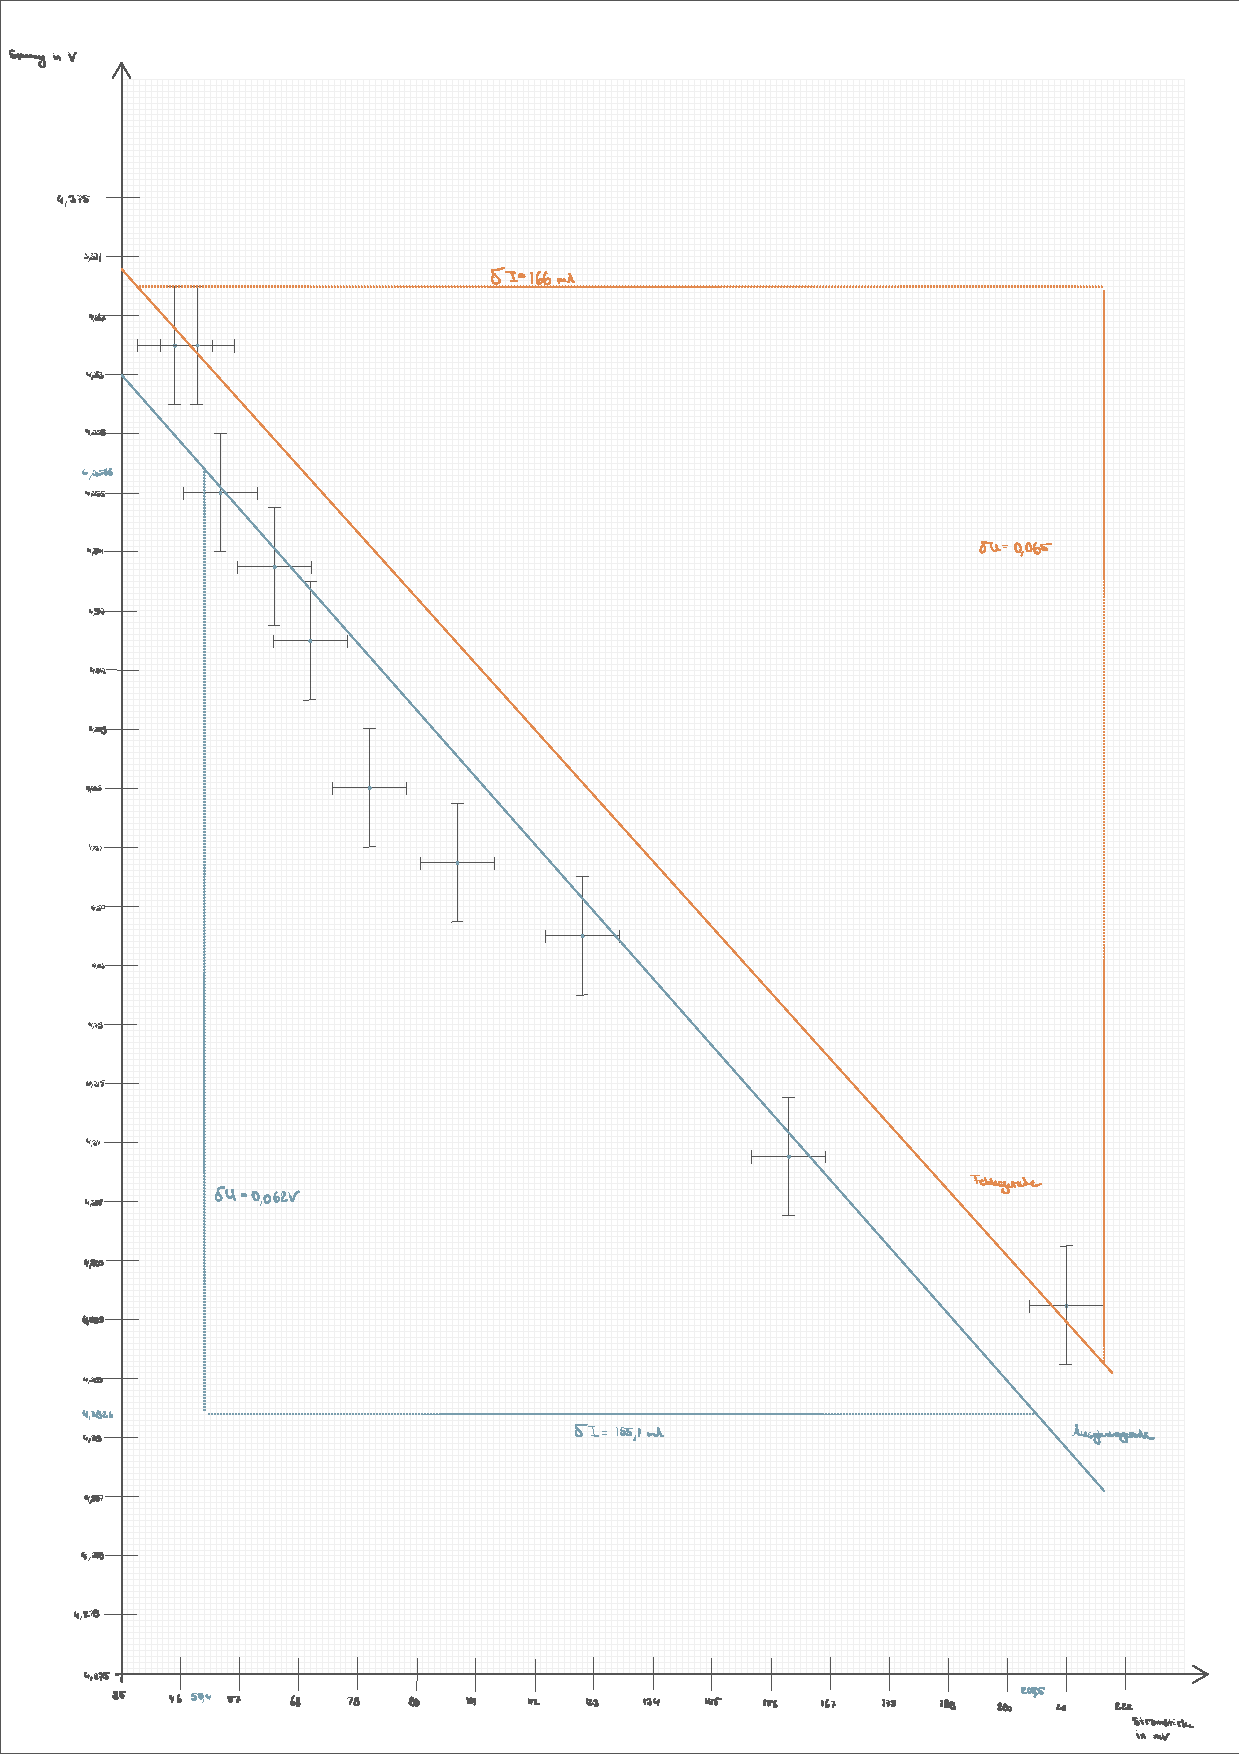
\includegraphics[width=1\textwidth]{img/23/plot-23-Strommessung.pdf}
    \caption{Spannung in Abhängigkeit der Stromstärke}
    \label{fig:u_i_diagramm}
\end{figure}
\twocolumn


\section{Bestimmung des Lastwiderstands für maximale Leistung}
Nun soll bestimmt werden, für welchen Lastwiderstand \(R_L\) die an den Last abgegebene
Leistung \(P=U_k I\) maximal ist. Es gilt:
\begin{equation}
    I=\frac{U_q}{R_i+R_L},
\end{equation}
woraus sich die an der Last abfallende Leistung als Funktion von \(R_L\) über \hyperref[eq:klemmenspannung]{Gleichung \ref*{eq:klemmenspannung}} ergibt:
\begin{equation}
    P(R_L)=U_q^2\frac{R_L}{(R_i+R_L)^2}.
\end{equation}

Zur Bestimmung eines Extrems wird die erste Ableitung nach \(R_L\) gebildet:
\begin{align*}
    \frac{\mathrm{d}P}{\mathrm{d}R_L}
    &=U_q^2\frac{\mathrm{d}}{\mathrm{d}R_L}\left(\frac{R_L}{(R_i+R_L)^2}\right)\\
    &=U_q^2\left(\frac{1}{(R_i+R_L)^2}-\frac{2R_L}{(R_i+R_L)^3}\right)\\
    &=U_q^2\frac{R_i-R_L}{(R_i+R_L)^3}.
\end{align*}
Setzt man \(\dfrac{\mathrm{d}P}{\mathrm{d}R_L}=0\), folgt unmittelbar
\begin{equation}
    R_L=R_i.
\end{equation}

Um sicherzustellen, dass es sich um ein Maximum handelt, wird die zweite Ableitung betrachtet   :
\begin{equation}
    \frac{\mathrm{d}^2P}{\mathrm{d}R_L^2}
    =2U_q^2\frac{R_L-2R_i}{(R_i+R_L)^4}.
\end{equation}
Für \(R_L=R_i\) ergibt sich
\begin{equation}
    \left.\frac{\mathrm{d}^2P}{\mathrm{d}R_L^2}\right|_{R_L=R_i}
    =-\frac{U_q^2}{8R_i^3}<0,
\end{equation}
also liegt tatsächlich ein Maximum vor.

Für \(R_L=R_i\) vereinfacht sich der Strom zu
\begin{equation}
    I=\frac{U_q}{2R_i},
\end{equation}
und die Klemmenspannung zu
\begin{equation}
    U_k=\frac{U_q R_L}{R_i+R_L}=\frac{U_q}{2}.
\end{equation}
Mit den gemessenen Werten ergibt sich
\begin{equation}
    \boxed{
        U_k=\frac{U_q}{2}=(2,122\pm 0,057)\,\mathrm{V}
    }.
\end{equation}